\documentclass[11pt,a4paper]{article}

% ------------------------------------------------------------------
% Packages
% ------------------------------------------------------------------
\usepackage[utf8]{inputenc}
\usepackage[T1]{fontenc}
\usepackage[english]{babel}
\usepackage{amsmath,amssymb}
\usepackage{geometry}
\geometry{margin=1.9cm, headheight=14pt}
\usepackage{booktabs}
\usepackage{array}
\usepackage{multirow}
\usepackage{graphicx}
\usepackage{xcolor}
\usepackage{fancyhdr}
\usepackage{caption}
\usepackage{subcaption}
\usepackage{siunitx}
\usepackage{enumitem}
\usepackage[hidelinks]{hyperref}
\usepackage{float}
\usepackage{pgfplots}
\pgfplotsset{compat=1.17}
\usepgfplotslibrary{groupplots}

% ------------------------------------------------------------------
% Styling
% ------------------------------------------------------------------
\pagestyle{fancy}
\fancyhf{}
\lhead{A* Password Cracker}
\rhead{Parallel \& Distributed Systems}
\cfoot{\thepage}

\sisetup{round-mode=places,round-precision=3}
\setlist{nosep}

% ------------------------------------------------------------------
% Title
% ------------------------------------------------------------------
\title{\vspace{-1.0cm}\textbf{Parallel A* Password Recovery} \\[2pt]
       \large Sequential, Pthreads, OpenMP, OpenCilk, CUDA and Hybrid CPU+GPU Implementations}
\author{Parallel \& Distributed Systems (Homework 4) \\ Apostolos Pantazis (10910)}
\date{October 2026}

\begin{document}
\maketitle
\thispagestyle{fancy}
\vspace{-0.9cm}

\begin{abstract}
\noindent We implement an MD5 password-recovery tool as a memory-bounded \textbf{A* state-space
search} over a prefix tree and parallelize it across five paradigms: POSIX threads, OpenMP,
OpenCilk, CUDA, and a Hybrid Pthreads\,+\,CUDA design. We study how wall-clock time scales with the
size of the problem --- both with the password length $L$ and with the volume of candidates the
search must process --- on a 28-core host with an NVIDIA RTX~4070~Ti~SUPER. Time grows essentially
linearly with the number of candidates processed and multiplies by roughly the alphabet size for
each additional character position. A single-threaded search cannot recover a length-5 target within
the $60$\,s budget, but every parallel variant does once given enough workers (Pthreads from $2$
threads, OpenMP/OpenCilk from $4$; pure CUDA completes at every tested batch size but is slowest),
with the Hybrid CPU+GPU design the fastest overall.
\end{abstract}

\vspace{-0.3cm}
% ==================================================================
\section{Problem Formulation}
% ==================================================================
Given the MD5 digest of an unknown password of known length $L$, we recover the plaintext. Because
cryptographic hashes exhibit the avalanche effect, there is no continuous ``distance'' between a
partial candidate and the target, so the hash does not guide the search. Instead we treat the
problem as a graph search over a prefix tree and use A* as a systematic, memory-bounded traversal.

\paragraph{State-space model.}
\textbf{State:} a candidate prefix $s$ at depth $d$. \textbf{Alphabet:} a fixed 76-symbol set
(lowercase, uppercase, digits, and \verb|!@#$%^&*()-_=+|). \textbf{Path cost:}
$g(n)=d\cdot\text{EDGE\_COST}$ with $\text{EDGE\_COST}=1$. \textbf{Heuristic:}
$h(n)=(L-d)\cdot\text{EDGE\_COST}$ (remaining depth; admissible and consistent). \textbf{Evaluation:}
$f(n)=g(n)+h(n)=L$, uniform across all candidates of the target length, so A* reduces to a
systematic frontier expansion steered toward leaves. \textbf{Goal test:} MD5 verification only when
a candidate reaches depth $L$. To bound memory we apply \textbf{beam trimming}: when the queue
exceeds $\texttt{BEAM\_CAP}=3{,}000{,}000$, a \texttt{quickselect} keeps the best
$\texttt{BEAM\_KEEP}=1{,}200{,}000$ in expected $O(n)$ and re-heapifies.

\paragraph{Problem size.}
A length-$L$ password is a point in a discrete space of $L$ coordinates, each drawn from the
76-symbol alphabet, so the search explores up to $76^{L}$ candidates: $76^{4}\approx3.34\times10^{7}$
at length 4 and $76^{5}\approx2.54\times10^{9}$ at length 5. The number actually processed before
recovery --- expanded nodes plus leaf verifications --- varies by target, since A* reaches different
leaves at different times. The two quantities that drive cost are therefore the password length and
the candidate volume, and adding one character multiplies the worst case by 76; we report runtime
against both below.

% ==================================================================
\section{Implementations (brief)}
% ==================================================================
All variants share a binary min-heap priority queue (\texttt{push}/\texttt{pop} in $O(\log n)$) with
quickselect beam-trim, and a dependency-free RFC~1321 MD5. The root space is decomposed into
$76^{2}=5{,}776$ two-character prefix tasks for $L\ge2$.
\begin{itemize}
  \item \textbf{Pthreads:} workers claim tasks via an atomic counter (\texttt{atomic\_fetch\_add});
        each owns a private heap (no lock contention); an atomic flag ends the search on a hit.
  \item \textbf{OpenMP:} same decomposition via \texttt{\#pragma omp parallel for schedule(dynamic,1)}
        with preallocated per-thread heaps.
  \item \textbf{OpenCilk:} \texttt{cilk\_for} exposes the sub-tasks to the work-stealing runtime;
        worker count set by \texttt{CILK\_NWORKERS}.
  \item \textbf{CUDA:} the CPU drives traversal/heap while completed leaves accumulate in a batch
        buffer; when full, the batch is hashed in parallel on the GPU. Here \texttt{--threads} is the
        GPU \emph{batch size}.
  \item \textbf{Hybrid Pthreads\,+\,CUDA:} each POSIX worker owns a CUDA stream, pinned host memory,
        and private device buffers/flags --- CPU task distribution overlapped with GPU batch hashing.
\end{itemize}

\paragraph{Setup.} 28 logical cores (WSL2, Linux~6.6); NVIDIA RTX~4070~Ti~SUPER (\texttt{sm\_89});
\texttt{gcc -O2}, OpenCilk \texttt{clang}, \texttt{nvcc -O3}. Budgets:
$\texttt{TIME\_BUDGET}=60$\,s, $\texttt{NODE\_BUDGET}=3.5\times10^{7}$. Timings are wall-clock for the
A* phase. Node counts vary slightly with thread count because the parallel frontier is
nondeterministic; this does not affect correctness.

% ==================================================================
\section{Execution Time vs.\ Number of Data Points}
% ==================================================================
At a fixed length, different targets are recovered after a different number of expanded nodes.
Figure~\ref{fig:datapoints} plots execution time against the number of data points processed, and
the relationship is essentially \textbf{linear}: cost is dominated by how many candidates the search
must touch, not by any per-candidate complexity. Both the sequential baseline (length 4) and the
Hybrid design (length 5, 16 threads) trace straight lines.

\begin{figure}[H]
\centering
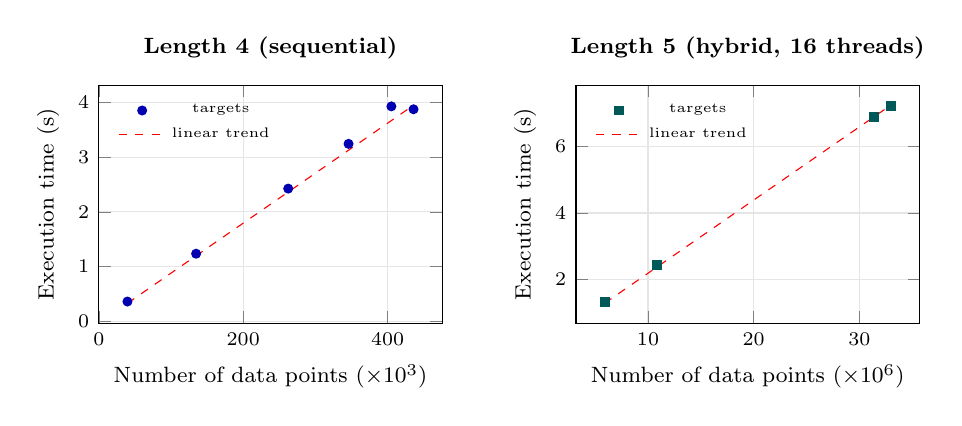
\begin{tikzpicture}
\begin{groupplot}[
  group style={group size=2 by 1, horizontal sep=1.7cm},
  width=0.49\textwidth, height=4.6cm,
  grid=both, grid style={gray!20},
  tick label style={font=\scriptsize}, label style={font=\footnotesize},
  title style={font=\footnotesize\bfseries},
]
% ---- D=4 sequential: time vs nodes (data points) ----
\nextgroupplot[title={Length 4 (sequential)},
  xlabel={Number of data points ($\times10^{3}$)}, ylabel={Execution time (s)},
  legend style={font=\tiny,at={(0.03,0.97)},anchor=north west,draw=none,fill=none}]
\addplot[only marks,mark=*,mark size=1.6pt,color=blue!70!black] coordinates {
 (39.680,0.362) (134.763,1.236) (262.264,2.426) (345.816,3.244) (405.146,3.929) (435.824,3.876)};
\addplot[no marks,dashed,color=red] coordinates {(39.680,0.330)(435.824,3.95)};
\legend{targets, linear trend}
% ---- D=5 hybrid: time vs nodes (data points) ----
\nextgroupplot[title={Length 5 (hybrid, 16 threads)},
  xlabel={Number of data points ($\times10^{6}$)}, ylabel={Execution time (s)},
  legend style={font=\tiny,at={(0.03,0.97)},anchor=north west,draw=none,fill=none}]
\addplot[only marks,mark=square*,mark size=1.6pt,color=teal!70!black] coordinates {
 (5.895,1.319) (10.894,2.430) (31.348,6.881) (32.955,7.224)};
\addplot[no marks,dashed,color=red] coordinates {(5.895,1.28)(32.955,7.25)};
\legend{targets, linear trend}
\end{groupplot}
\end{tikzpicture}
\caption{Execution time grows linearly with the number of data points (nodes) processed, at both
lengths. Left: six length-4 targets, sequential. Right: four length-5 targets, Hybrid at
16 threads (batch $65{,}536$).}
\label{fig:datapoints}
\end{figure}

\vspace{-0.3cm}
\paragraph{CPU scaling at length 4.} Table~\ref{tab:len4} gives representative times. Adding threads
distributes the work across cores; Pthreads and OpenMP scale near-linearly, while OpenCilk's
work-stealing reorders leaf exploration, making it fast on some targets and slower on others.

\begin{table}[H]
\centering
\caption{Wall-clock time (s) at length 4 (search space $76^{4}$). \textit{seq} single-threaded;
parallel columns use the stated thread count; CUDA uses batch $262{,}144$.}
\label{tab:len4}
\small
\begin{tabular}{@{}lrrrrrrr@{}}
\toprule
\textbf{Target} & \textbf{seq} & \textbf{pth-8} & \textbf{pth-32} & \textbf{omp-8} & \textbf{omp-32} & \textbf{cilk-8} & \textbf{cuda} \\
\midrule
PtYg  & 0.362 & 0.253 & 0.097 & 0.593 & 0.200 & 0.162 & 0.130 \\
j\&mU & 1.236 & 0.060 & 0.027 & 0.145 & 0.051 & 0.021 & 0.423 \\
=h\#B & 2.426 & 0.483 & 0.184 & 1.029 & 0.360 & 0.383 & 0.891 \\
el31  & 3.244 & 0.027 & 0.012 & 0.062 & 0.022 & 0.228 & 1.054 \\
iEl(  & 3.929 & 0.054 & 0.022 & 0.117 & 0.041 & 0.363 & 1.156 \\
2h-p  & 3.876 & 0.342 & 0.130 & 0.769 & 0.249 & 0.328 & 1.364 \\
\bottomrule
\end{tabular}
\end{table}

\vspace{-0.3cm}
\paragraph{Throughput vs.\ threads.} Table~\ref{tab:speedup} reports Pthreads self-relative speedup
for \texttt{PtYg}: more threads explore the frontier in parallel, giving super-linear speedup at
4--8 threads (the target leaf is reached out-of-order, earlier than a serial scan), falling to
$68\%$ efficiency at 32 threads due to overhead and saturation.

\begin{table}[H]
\centering
\caption{Pthreads self-relative speedup, target \texttt{PtYg}, length 4 (baseline 1 thread: 2.106\,s).}
\label{tab:speedup}
\small
\begin{tabular}{@{}rrrr|rrrr@{}}
\toprule
\textbf{Thr.} & \textbf{Time} & \textbf{Speedup} & \textbf{Eff.} &
\textbf{Thr.} & \textbf{Time} & \textbf{Speedup} & \textbf{Eff.} \\
\midrule
1 & 2.106 & 1.00$\times$ & 100\% & 8  & 0.253 & 8.32$\times$  & 104\% \\
2 & 1.075 & 1.96$\times$ & 98\%  & 16 & 0.150 & 14.04$\times$ & 88\%  \\
4 & 0.520 & 4.05$\times$ & 101\% & 32 & 0.097 & 21.71$\times$ & 68\%  \\
\bottomrule
\end{tabular}
\end{table}

% ==================================================================
\section{Execution Time vs.\ Number of Dimensions}
% ==================================================================
Going from length 4 to length 5 adds one dimension and multiplies the worst-case candidate count by
$76\times$. The effect on execution time is shown in Figure~\ref{fig:dims} (note the
\emph{logarithmic} time axis). At length 4 every variant recovers the target in well under a second.
At length 5 the picture splits by \emph{degree of parallelism}, not by paradigm: the single-threaded
Sequential search exhausts the $60$\,s budget, whereas each parallel variant recovers the target once
it has enough workers --- Pthreads already at $2$ threads, OpenMP and OpenCilk from $4$, while pure
CUDA completes at every tested batch size (slowest of all). The Hybrid design is simply the fastest, overlapping
multi-threaded frontier expansion with asynchronous GPU leaf-verification; it is not the only variant
that completes length 5. These length-5 numbers are all for target \texttt{yJuq)}
(Table~\ref{tab:len5sweep}); completion at length 5 is target-dependent, so a harder target can still
drive the low-thread CPU runs to the budget wall.

\begin{figure}[H]
\centering
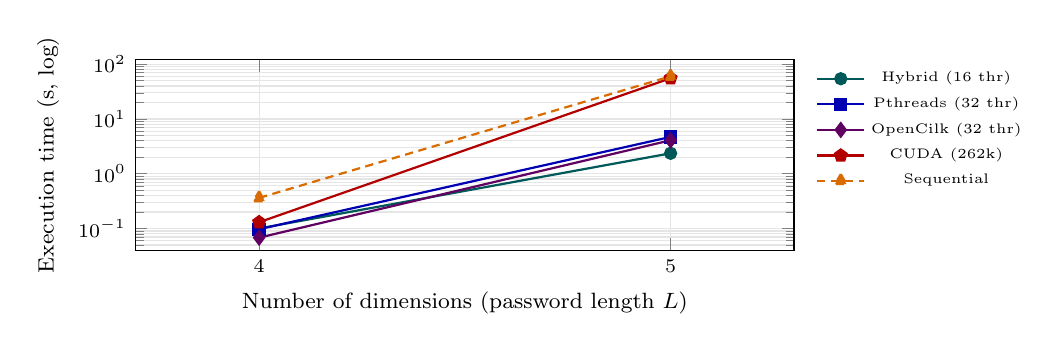
\begin{tikzpicture}
\begin{axis}[
  width=0.82\textwidth, height=4.0cm,
  xlabel={Number of dimensions (password length $L$)},
  ylabel={Execution time (s, log)}, ymode=log,
  xtick={4,5}, xmin=3.7, xmax=5.3,
  grid=both, grid style={gray!20},
  tick label style={font=\scriptsize}, label style={font=\footnotesize},
  legend style={font=\tiny, at={(1.02,1.0)}, anchor=north west, draw=none},
  ymin=0.04, ymax=120,
]
% Hybrid 16 threads: L4 PtYg=0.100 (hybrid_report.txt random_a) ; L5 yJuq) batch 262144 = 2.358
\addplot[mark=*,mark size=2pt,color=teal!70!black,thick] coordinates {(4,0.100) (5,2.358)};
% Pthreads (32 thr): L4 PtYg=0.097 ; L5 yJuq) = 4.70 (found)
\addplot[mark=square*,mark size=2pt,color=blue!70!black,thick] coordinates {(4,0.097) (5,4.70)};
% OpenCilk (32 thr): L4 PtYg=0.068 ; L5 yJuq) = 4.08 (found)
\addplot[mark=diamond*,mark size=2.4pt,color=violet!75!black,thick] coordinates {(4,0.068) (5,4.08)};
% CUDA (batch 262144): L4 PtYg=0.130 ; L5 yJuq) = 55.39 (found)
\addplot[mark=pentagon*,mark size=2.2pt,color=red!70!black,thick] coordinates {(4,0.130) (5,55.39)};
% Sequential: L4 PtYg=0.362 ; L5 yJuq) DNF -> 60.046 (budget cap)
\addplot[mark=triangle*,mark size=2.4pt,color=orange!85!black,thick,densely dashed] coordinates {(4,0.362) (5,60)};
\legend{Hybrid (16 thr), Pthreads (32 thr), OpenCilk (32 thr), CUDA (262k), Sequential}
\end{axis}
\end{tikzpicture}
\caption{Execution time vs.\ number of dimensions (log time axis), length-5 target \texttt{yJuq)}
(length-4 points use \texttt{PtYg}). One added dimension is a $76\times$ growth in the search space.
Only the single-threaded Sequential search hits the 60\,s budget at length 5 (dashed, plotted at the
cap; recovery fails). Every parallel variant recovers the target: Pthreads and OpenCilk in a few
seconds at 32 threads, pure CUDA in $\approx\!55$\,s at a $262{,}144$ batch, and the Hybrid design
fastest at $\approx\!2.4$\,s (16 threads, $262{,}144$ batch).}
\label{fig:dims}
\end{figure}

\vspace{-0.2cm}
\paragraph{Length-5 thread scaling (CPU variants).} Table~\ref{tab:len5sweep} gives the full
thread sweep on \texttt{yJuq)}. Every variant DNFs at $1$ thread, but the CPU-parallel ones recover
as soon as a few workers share the search (Pthreads at $2$, OpenMP/OpenCilk at $4$); time then falls
roughly linearly --- Pthreads from $49.6$\,s to $4.7$\,s ($2\!\to\!32$ threads) --- with noise from
\emph{when} a worker hits the target leaf. Pure CUDA stays slowest and essentially flat across batch
sizes ($54.8\!\to\!51.9$\,s for a $64\times$ larger batch): the serial CPU frontier, not GPU hashing,
starves the device, so a bigger batch barely helps.

\begin{table}[H]
\centering
\caption{Length-5 wall-clock time (s) on target \texttt{yJuq)} (budget $60$\,s; ``DNF'' = budget
exhausted before recovery). Columns are CPU worker threads. Sequential is single-threaded; CUDA and
Hybrid are reported below the table since their knob is the GPU batch size.}
\label{tab:len5sweep}
\small
\begin{tabular}{@{}lrrrrrr@{}}
\toprule
\textbf{Variant} & \textbf{1} & \textbf{2} & \textbf{4} & \textbf{8} & \textbf{16} & \textbf{32} \\
\midrule
Pthreads & DNF & 49.59 & 24.45 & 12.20 & 7.50 & 4.70 \\
OpenMP   & DNF & DNF   & 42.84 & 26.10 & 15.10 & 8.73 \\
OpenCilk & DNF & DNF   & 22.10 & 2.92 & 21.51 & 4.08 \\
\midrule
\multicolumn{7}{@{}l}{\emph{Sequential}: DNF (single-threaded, $60.00$\,s cap).}\\
\multicolumn{7}{@{}l}{\emph{CUDA} (GPU batch, all \emph{found}): $65{,}536$ $54.76$; $262{,}144$ $55.39$; $1{,}048{,}576$ $52.45$; $4{,}194{,}304$ $51.91$.}\\
\multicolumn{7}{@{}l}{\emph{Hybrid} ($16$ thr, batch $262{,}144$): $2.36$ --- fastest overall (cf.\ Table~\ref{tab:hyb5}).}\\
\bottomrule
\end{tabular}
\end{table}

\vspace{-0.2cm}
\paragraph{Hybrid at length 5.} Table~\ref{tab:hyb5} sweeps the GPU batch size at 16 threads for the
four length-5 targets. All are recovered. Larger batches amortize kernel-launch overhead over more
candidates per launch, cutting both launch count and time; the knee sits around
$262{,}144$--$1{,}048{,}576$. At a single thread the Hybrid exhausts the budget just like the other
variants; its advantage is that, once threads cooperate, it reaches recovery faster than any CPU-only
variant (e.g.\ $2.4$\,s vs.\ Pthreads' $4.7$\,s on \texttt{yJuq)}) by overlapping CPU frontier
expansion with asynchronous GPU verification.

\begin{table}[H]
\centering
\caption{Hybrid batch-size sweep, 16 threads, length 5 (search space $76^{5}\approx2.54\times10^{9}$). All \emph{found}.}
\label{tab:hyb5}
\small
\begin{tabular}{@{}lrrr@{\hskip 1.2em}lrrr@{}}
\toprule
\textbf{Target} & \textbf{Batch} & \textbf{Time (s)} & \textbf{Nodes} &
\textbf{Target} & \textbf{Batch} & \textbf{Time (s)} & \textbf{Nodes} \\
\midrule
\multirow{4}{*}{yJuq)}
 & 16\,384   & 3.056 & 10\,857\,302 & \multirow{4}{*}{(K5cq} & 16\,384   & 8.522 & 31\,350\,410 \\
 & 65\,536   & 2.433 & 10\,880\,545 &                        & 65\,536   & 6.937 & 31\,383\,357 \\
 & 262\,144  & 2.358 & 10\,911\,899 &                        & 262\,144  & 6.814 & 31\,381\,106 \\
 & 1\,048\,576 & 2.350 & 10\,994\,144 &                      & 1\,048\,576 & 6.922 & 31\,458\,800 \\
\midrule
\multirow{4}{*}{ntG0y}
 & 16\,384   & 1.683 & 5\,896\,277 & \multirow{4}{*}{=e!4f}  & 16\,384   & 9.242 & 32\,983\,733 \\
 & 65\,536   & 1.383 & 5\,910\,865 &                         & 65\,536   & 7.394 & 32\,987\,203 \\
 & 262\,144  & 1.315 & 5\,920\,023 &                         & 262\,144  & 7.155 & 32\,953\,977 \\
 & 1\,048\,576 & 1.349 & 6\,003\,289 &                       & 1\,048\,576 & 7.279 & 33\,120\,763 \\
\bottomrule
\end{tabular}
\end{table}

% ==================================================================
\section{Discussion and Conclusion}
% ==================================================================
\textbf{Candidate volume.} Wall-clock time is a near-linear function of how many candidates the
search actually processes (Fig.~\ref{fig:datapoints}); parallelism reduces time by splitting that
work across cores, with super-linear speedups when a worker reaches the target leaf early.
\textbf{Length.} Each added character multiplies the search space by the alphabet size
(76$\times$), which is why length 4 is trivial for the CPU but length 5 saturates it
(Fig.~\ref{fig:dims}). \textbf{Where the GPU pays off.} At length 4 pure CUDA rarely beats a
well-parallelized CPU because the bottleneck is CPU-side frontier expansion, not hashing; at length 5
pure CUDA does recover the target but remains the slowest of the completing variants ($\approx\!52$--$55$\,s
on \texttt{yJuq)}), since its single-threaded frontier, not the hashing, is the limit --- which is
exactly what the Hybrid design fixes by expanding the frontier on many CPU threads at once.
\textbf{Batch
size.} Small batches ($16{,}384$) drown in launch overhead; $262{,}144$--$1{,}048{,}576$ minimize
launches per candidate and give the best time. \textbf{Oversubscription.} At 32 threads several
Hybrid cases show a jump in nodes and time as GPU contention and frontier divergence outweigh added
CPU parallelism.

\medskip
\noindent In summary, all six implementations are correct and reproducible. Time scales linearly with
candidate volume and multiplicatively with length; at length 4 the CPU variants reach
$\approx21\times$ speedup (Pthreads, 32 threads). At length 5 the decisive factor is the degree of
parallelism, not the paradigm: a single thread exhausts the budget while every parallel variant
recovers the target, with the Hybrid design fastest ($\approx\!2.4$\,s vs.\ $\approx\!4.1$\,s for the best
CPU-only variant on \texttt{yJuq)}).

\vspace{0.4em}
\noindent\textbf{You can find all the necessary files for this project on this GitHub repository:} \\
\url{https://github.com/pantazisa/Homework/tree/main/Homework%204}

\end{document}